\documentclass{beamer}
\usetheme{Singapore}

%Import from: http://tex.stackexchange.com/questions/58092/how-do-i-fit-java-style-source-code-in-one-frame-in-beamer
\usepackage{listings}
\usepackage{booktabs}
\lstset{language=Java,
                basicstyle=\footnotesize\ttfamily,
                keywordstyle=\footnotesize\color{blue}\ttfamily,
}

\title[SIDH]{Efficiency of SIDH/Isogeny Signatures}
\author{Robert Gorrie}
\institute[Comp Sci 2S03]{Department of Computing \& Software, McMaster University}
\date{November 16th, 2017}

\begin{document}

\begin{frame}
\titlepage
\end{frame}

\begin{frame}
\frametitle{Table of Contents}
\tableofcontents
\end{frame}

\AtBeginSection[]{
\begin{frame}<beamer>
\frametitle{Table of Contents}
\tableofcontents[currentsection]
\end{frame}
}

\section{Isogeny Based Signatures}

%high level signature description via fiat-shamir

\begin{frame}
\frametitle{Current Performance of SIDH}
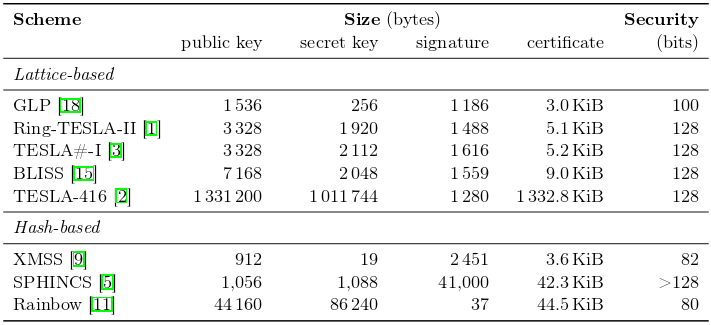
\includegraphics[scale=0.43]{sigcomparison.png}
\end{frame}

\begin{frame}
\frametitle{Isogeny Based Signatures}
\begin{itemize}
\item Yoo et. al provide an isogeny based signature scheme built off the Microsoft SIDH 1.0 Library.
\item The scheme is constructed using the ZKPoK 
\end{itemize}
\end{frame}

\begin{frame}
\frametitle{Performance of Isogeny Signatures}
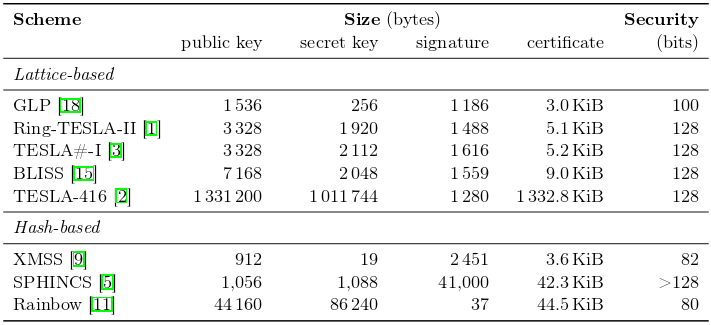
\includegraphics[scale=0.43]{sigcomparison.png}
\end{frame}

\section{Inversion Batching}

%before this, background on inversions in sidh/sig
\begin{frame}[fragile]
\frametitle{Batched Inversion Procedure}
\begin{itemize}
\item<1-> 1
\item<2-> 2
\item<3-> 3
\end{itemize}
%equation for inverting two elements, shamir?
%operation count reduction
\end{frame}

\begin{frame}
\frametitle{Performance Increase}
\begin{center}
\begin{tabular}{@{}lllll@{}}
	\toprule
	Procedure & Without Batching & With Batching\\
	\midrule
	Signature Sign & 15.74 & 15.56\\
	Sign Parallel & 10.23 & 10.13\\
	Signature Verify & 11.18 & 10.8\\
	Verify Parallel & 7.27 & 7.11\\
	\bottomrule
\end{tabular}\\
Measured in billions of clock cycles
\end{center}

\end{frame}

\section{Signature Compression}

\begin{frame}
\frametitle{SIDH Key Compression}

\end{frame}

\begin{frame}
%goal
\frametitle{Signature Compression}
\begin{center}
%\includegraphics[scale=0.65]{code5.png}
\end{center}
\end{frame}

%preliminary results
\begin{frame}
\frametitle{Results}
\end{frame}

\section{Additional Work}

\begin{frame}
\frametitle{}

\begin{center}
%\includegraphics[scale=0.65]{code5.png}
\end{center}
\end{frame}

\end{document}
